\section{Theoretische Grundlage}
\label{sec:Theorie}
Ziel des Versuches ist es die innere Abschirmungszahlen verschiedener Alkali-Metalle anhand derer Emissionslinien zu bestimmen.
Alakli-Metalle bestizen nur komplett besetzte Schalen und  ein Valenzelektronen. Diese lassen sich mit Hilfe der Ein-Elektronen-Näherung recht einfach beschreiben. Der Anatz der Näherungberuht darauf, das die Ladungen der Elektronen welche die kompletten Schalen besetzen sich mit denen, der Protonen des Kerns kompensiert. Somit kann das Atom als Wasserstoffatom genähert werden. Das zwischen dem Proton und Neutron liegende Columbfeld, wird durch die inneren Elektronen abgeschirmt. Dies wird im weiteren Verlauf der Rechnung durch die Abschirmzahl $\sigma$ berücksichtigt.
\begin{equation}
  z_\text{eff} = z - \sigma
  \label{eqn:zeff}
\end{equation}
Somit errechnet sich die effiktive Anzahl von Protonen entsprechend Gleichung \eqref{eqn:zeff}.
Um die Energieeigenwerte des Symstems zu berchnen wird zunächst die Schrödingergleichung aufgestellt,
\begin{equation}
  \left( \sum_\text{i} \frac{P_\text{i}^2}{2 m_\text{i}} + U \right) \Psi = E \Psi
  \label{eqn:Sch}
\end{equation}
für die sich die Lösungen
\begin{equation}
  E(n) = R_{\infty} \frac{1}{n^2}, \. n =1, \, 2, \, \cdots
  \label{eqn:En}
\end{equation}
ergeben. Dabei ist $n$ die Hauptquantenzahl. Da es sich jedoch um ein Kugelsymetrisches Problem handelt muss zunächst noch der Laplaceoperator in Kugelkoordinaten eingeführt werden. Zusätzlich wird nun beim Potential die Abschirmkonstante berücksichtigt, so dass sich das Potential der Form
\begin{equation}
  U = - \frac{\left( z - \sigma \right) e_0^2}{4 \pi  \varepsilon_0 r}
  \label{schrö}
\end{equation}
ergibt. Die Lösung der für das an das System angepasste Schrödingergleichung wird relativistisch betrachtet und in einer Potenzreihe umgeschrieben so dass sich die Energieigenwerte
\begin{equation}
  E_\text{rel n,l} = -R_{\infty} \left( \frac{(z - \Sigma)^2}{n²} + \alpha^2 \frac{(z - \sigma)^4}{n^3}\left( \frac{2}{2 l +1} - \frac{3}{4n} \right) \right)
  \label{eqn:ham}
\end{equation}
ergeben. Dabei entspricht $\alpha$ der Sommerfeldschen Feinstrukturkonstante , $R_{\infty}$ der Rydbergenergie
\begin{equation}
  \alpha := \frac{e_0^2}{2 h c \varepsilon_0}
  \label{eqn:alpha}
\end{equation}
und $l$ ist die Bahndrehquantenzahl die beim lösen der Schrödingergleichung aus der Kugelflächenfunktion resultiert.
Desweiteren muss die Spin-Bahn-Kopplung $S$ der Elektronen berücksichtigt werden. Sie ist neben dem aus den kugelsymetrischen Laplaceoperator folgender Drehimpuls $L$ ein weiterer. Mittels Störungstheorie wird der Einflusses des Spins berechnet. Es ergibt sich die Energieeigenwertgleichung
\begin{equation}
  E_\text{n,j} = -R_{\infty}\left( \frac{(z - \Sigma)^2}{n²} + \alpha^2 \frac{(z - \sigma)^4}{n^3} \left( \frac{1}{j + 0.5} - \frac{3}{4n} \right) \right)
  \label{<++>}
\end{equation}
wobei die Spinquantenzahl $j$ nur die Werte $l + \frac{1}{2}$ und $l - \frac{1}{2}$ annehmen kann.

Angeregte Valenzelektronen haben bei den durch die "Quantenzahlen $n ,l$ und $j$ gekennzeichneten Energieniveaus verschiedene Übergangswahrscheinlichkeiten".	Die entsprechende Bahndrehquantenzahl $l$ ändert sich jeweils um $\delta l$ = $\pm 1$. Darüber hinaus ist ein Übergang der Spinquantenzahl $\delta j = 0$ zwar möglich, aber sehr unwahrscheinlich. Die Hauptquantenzahl n ist nicht eingeschränkt, wird jedoch mit steigendem n immer unwahrscheinlicher. Das Phänomen das bei gleicher Bahndrehquantenzahl und unterschiedlichen Spinquantenzahlen wei Spektrallinien dicht beieinadner liegen,wird als Doublett-Struktur bezeichnet. In Abbildung \ref{fig:ene} ist ein Beispiel für verschiedene Energieniveaus abgebildet.
\begin{figure}
  \centering
  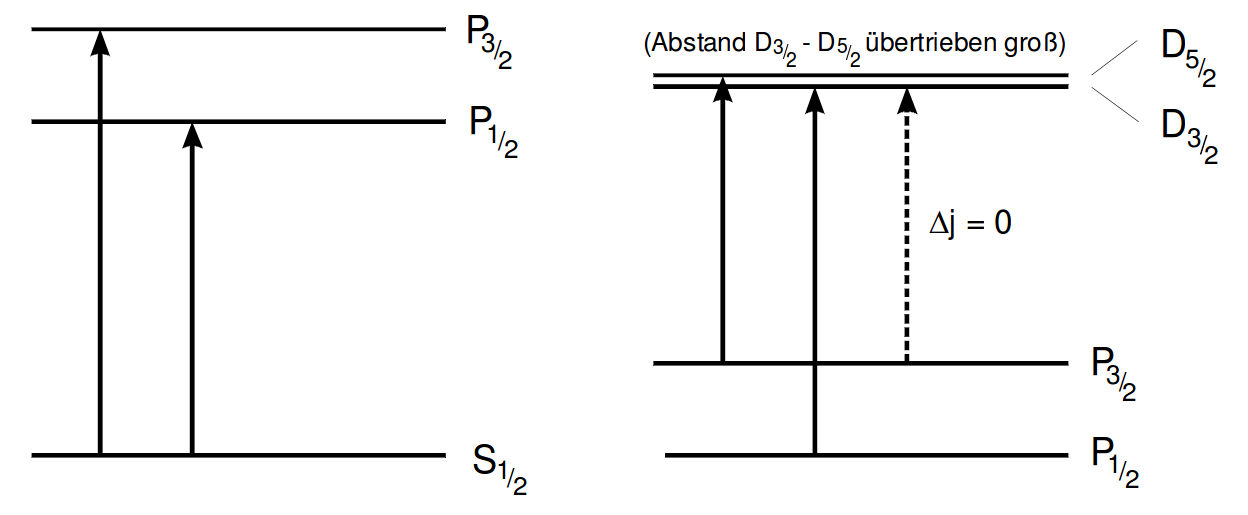
\includegraphics[height=6cm]{picture/eniv.png}
  \caption{Beispiel für Energieniveaus der Spektrallinien \cite{sample}}
  \label{fig:ene}
\end{figure}

Um Schlussendlich die Energie des Leuchtelektron genau zu bestimmen wird die Abschirmkonstante in zwei Teile eingeteilt. Einerseits in die Konstante der vollen Abschirmung $\sigma_1$ und der der inneren Abschirmung $\sigma_2$. Da die zweite Abschirmungskonstante $\sigma_2$ ausschließlich die vollbesetzten Unterschalen beschreibt unterscheidet ist diese nur geringfügig kleiner, als die volle Abschirmungskonstante $\sigma_1$ welche die Abschirmung aller Elektronen  impliziert. Als Dublett wird ein Quantenmechanischer Zustand bezeichnet bei dem sich lediglich die Quantenzahl $j$ von dem des anderen Zustandes um 1 unterscheidet. Anhand der Energiediffernz $\Delta E_\text{D}$ von Dubletts lässt sich die Abschirmungszahl $\sigma_2$ mit Gleichung \eqref{eqn:ded} bestimmen,
\begin{equation}
  \Delta E_\text{D} = \frac{R_{\infty} \alpha^2}{n^3} \left( z - \sigma_2 \right)^2 \frac{1}{l(l+1)}
  \label{eqn:ded}
\end{equation}
indem die Gleichung nach der Abschirmkonstante aufgelöst wird. Um die Energiedifferenz zu bestimmen wird anhand des Wellenlängenunterschied der beiden Spektrallinien des Dubletts entsprechend der Gleichung
\begin{equation}
  \Delta E_\text{D} = hc\left( \frac{1}{\lambda} - \frac{1}{\lambda'} \right)
  \label{eqn:ed}
\end{equation}
bestimmt.
Mit Hilfe der Interferenz an einem Gitter werden die Spektralien in ihre einzelnen Wellenlängen aufgespalten. Kunstruktive Interferens wird bei den Maximums $k$ter Ordung unter dem Winkel $\varphi$ beobachtet. Die Gitterkonstante wird als $g$ bezeichnet.
\begin{equation}
  sin \, \varphi = k \frac{\lambda}{g}
  \label{eqn:phi}
\end{equation}
Für die Bestimmung der Wellenlängenunterschied der Dubletts das Okularmikrometer geeicht werden. Näheres zu dem Verfahren wird in der Durchführung erwähnt. Aus Trigonometrischen Überlegungegen ergibt sich die Formel
\begin{equation}
  \delta\lambda = \frac{cos \, \varphi}{cos \, \varphi_{1,2}} \frac{\Delta s}{\Delta t}\left( \lambda_1 - \lambda_2 \right) \ .
  \label{eqn:dlam}
\end{equation}
$\varphi$ entspricht dem gemittelten Winkel der Doublettlinien und $\varphi_{1,2}$ die gemittelte Differenz der Douplettlinien. $\Delta s$ ist der Abstand zwischen den beiden Doublettlinien und $\Delta t$ der, der beiden bekannten Spektrallinien $\lambda_1$ und $\lambda_2$.

\subsection{Fehlerrechnung}
Sämtliche Fehlerrechnungen werden mit Hilfe von Python 3.4.3 durchgeführt.
\subsubsection{Mittelwert}
Der Mittelwert einer Messreihe $x_\text{1}, ... ,x_\text{n}$ lässt sich durch die Formel
\begin{equation}
	\overline{x} = \frac{1}{N} \sum_{\text{k}=1}^\text{N} x_k
	\label{eqn:ave}
\end{equation}
berechnen. Die Standardabweichung des Mittelwertes beträgt
\begin{equation}
	\Delta \overline{x} = \sqrt{ \frac{1}{N(N-1)} \sum_{\text{k}=1}^\text{N} (x_\text{k} - \overline{x})^2}
	\label{eqn:std}
\end{equation}

\subsubsection{Gauß'sche Fehlerfortpflanzung}
Wenn $x_\text{1}, ..., x_\text{n}$ fehlerbehaftete Messgrößen im weiteren Verlauf benutzt werden, wird der neue Fehler $\Delta f$ mit Hilfe der Gaußschen Fehlerfortpflanzung angegeben.
\begin{equation}
	\Delta f = \sqrt{\sum_{\text{k}=1}^\text{N} \left( \frac{ \partial f}{\partial x_\text{k}} \right) ^2 \cdot (\Delta x_\text{k})^2}
	\label{eqn:var}
\end{equation}

\subsubsection{Lineare Regression}
Die Steigung und y-Achsenabschnitt einer Ausgleichsgeraden werden gegebenfalls mittels Linearen Regression berechnet.
\begin{equation}
	y = m \cdot x + b
	\label{eqn:reg}
\end{equation}
\begin{equation}
	m = \frac{ \overline{xy} - \overline{x} \overline{y} } {\overline{x^2} - \overline{x}^2}
	\label{eqn:reg_m}
\end{equation}
\begin{equation}
	b = \frac{ \overline{x^2}\overline{y} - \overline{x} \, \overline{xy}} { \overline{x^2} - \overline{x}^2}
	\label{eqn:reg_b}
\end{equation}
